%%%%%%%%%%%%%%%%%%%%%%%%%%%%%%%%%%%%%%%%%%%%%%%%%%%%%%%%%%%%%%%%%%%%%%%%%%%%%%%%                     
%2345678901234567890123456789012345678901234567890123456789012345678901234567890
%        1         2         3         4         5         6         7         8

\documentclass[letterpaper, 10 pt, conference]{ieeeconf}  % Comment this line out
                                                          % if you need a4paper
%\documentclass[a4paper, 10pt, conference]{ieeeconf}      % Use this line for a4
                                                          % paper

\IEEEoverridecommandlockouts                              % This command is only
                                                          % needed if you want to
                                                          % use the \thanks command
\overrideIEEEmargins
% See the \addtolength command later in the file to balance the column lengths
% on the last page of the document




% The following packages can be found on http:\\www.ctan.org
%\usepackage{graphics} % for pdf, bitmapped graphics files
%\usepackage{epsfig} % for postscript graphics files
%\usepackage{mathptmx} % assumes new font selection scheme installed
%\usepackage{times} % assumes new font selection scheme installed
%\usepackage{amsmath} % assumes amsmath package installed
%\usepackage{amssymb}  % assumes amsmath package installed
\usepackage{csquotes}
\usepackage{graphicx}

\title{\LARGE \bf Image Reduction \& Classification}
\author{David Anderton and Ray Dedhia}


\begin{document}


\maketitle
\thispagestyle{empty}
\pagestyle{empty}


%%%%%%%%%%%%%%%%%%%%%%%%%%%%%%%%%%%%%%%%%%%%%%%%%%%%%%%%%%%%%%%%%%%%%%%%%%%%%%%%
\begin{abstract}

As the use of artificial intelligence continues to expand into the realm of image compression\footnote{https://ai.googleblog.com/2016/09/image-compression-with-neural-networks.html}\footnote{http://www.wave.one/icml2017/} questions are raised on how well the original artefacts and nature of the source image are preserved. The consequence of being able to utilize smaller output images, that maintain the majority of pertinent information, from their often 10 times larger source is huge. With smaller inputs applications from self driving cars that rely on camera input, autonomous flight, through to training neural nets could require significantly less processing time and resources.
In this paper, we briefly examine how the Google Cloud Vision API responds to the content of a selection of images pre- and post-compression. We also consider a variety of compression techniques and extents. The goal: produce a broad estimate of how much an image can be compressed until the Google Cloud Vision API, as a proxy for other classification algorithms, can no longer determine useful insights about the constitution of the image.

An interactive exploration of the results is available at the following URI: https://mit18065-dimensions.herokuapp.com/

\end{abstract}

%%%%%%%%%%%%%%%%%%%%%%%%%%%%%%%%%%%%%%%%%%%%%%%%%%%%%%%%%%%%%%%%%%%%%%%%%%%%%%%%
\section{INTRODUCTION}

In this paper, we briefly examine how the Google Cloud Vision API responds to the content of a selection of images pre- and post-compression. We also consider a variety of compression techniques and extents. The goal: produce a broad estimate of how much an image can be compressed until the Google Cloud Vision API, as a proxy for other classification algorithms, can no longer determine useful insights about the constitution of the image.

\section{METHODOLOGY}
Our methodology was as follows:

Within our study we utilised 22 unique images, from four major
categories: six animals, six famous landmarks, five landscapes, five
street signs. Expanding this to both the color and grayscale
versions of these images, we had a resulting set of 44 source images.

After collating the source images we sent them through the Google Cloud Vision API\footnote{The Google Cloud Vision API, https://cloud.google.com/vision/, classifies images into categories and detects objects and faces in images utilising non-public machine learning models.}
and get a control set of labels for the 44 images. Then compress the images, using the five following methods:
(1) Posterization through k-means clustering,
(2) :ow-rank approximation using Principle Component Analysis,
(3) \textquote{Mean pooling} operation commonly used in neural networks,
(4) Mogrify (a command-line utility)
and (5) Dropout (randomly removing a specific percentage of the pixels).

Once the images were compressed in all of the above methods we then re-queried the Google Cloud Vision API to re-classify the images post-compression and considered the results.

\section{COMPRESSION METHODS}
\subsection{Posterization}
K-means clustering is an algorithm that groups
a set of data points into $k$ groups by mapping each data point
to one of $k$ centroids such that the distance between each data point
and its centroid is minimized. It does this by randomly generating $k$
centroids, (1) assigning each data point to the nearest centroid,
(2) updating the centroid values be setting them equal to the arithmetic
mean of the data points assigned to them in step 1, and repeating steps
1 and 2 until some stopping criteria has been met. The resulting k-means clustering implemented a posterization
effect.

We arbitrarily stopped our k-means clustering algorithm after 10 iterations as an intuitive stopping point for efficiency, and used $k=4$ and $k=8$. In figure 1 below are the results of putting an image of a cat through 4-means and 8-means
clustering.

\vspace*{3mm}
\begin{tabular}{c c}
	\includegraphics[width=0.2\textwidth]{postfour} &
		\includegraphics[width=0.2\textwidth]{posteight} \\
	$k=4$ & $k=8$ \\
\end{tabular}

\subsection{Principle Component Analysis}
The principle components of some matrix, $M$, are its left and right singular vectors, $u_i$ and $v_i$ respectively, and its singular values,$sigma$. The decomposition of a matrix into these components is referred to most commonly as the Singular Value Decomposition, or SVD.
Principle Component Analysis, or PCA, is a form of matrix analysis that utilizes the largest principle components of a matrix of data in order to create a summarization or approximate the underlying data.

By utilising the Eckart-Young theorem\footnote{See Golub et al. https://www.ime.usp.br/~jstern/miscellanea/seminario/Golub87.pdf}, the rank $k$ matrix $M_k$ closest to $M$ is the sum of the product of the $k$ largest singular values of $M$with their corresponding left and right singular vectors. That is, $M_k = \sum_{i=1}^k \sigma_i u_i v_i^T$.

Thus, PCA can be utilised to find the best low-rank approximation for $M$.
Within our study we used PCA to reduce our image matrices to rank-5, rank-10 and rank-25 matrices.
In figure 2 below we can see the visual effect of calculating the best rank-5, rank-10 and rank-25
approximations of an image of Tokyo Tower.

\vspace*{3mm}
\begin{tabular}{c c c}
	\includegraphics[width=0.13\textwidth]{pcafive} &
		\includegraphics[width=0.13\textwidth]{pcaten} &
		\includegraphics[width=0.13\textwidth]{pcatwentyfive} \\
	rank-5 & rank-10 & rank-25 \\
\end{tabular}

\subsection{Mean Pooling}
Mean pooling refers to the operation of dividing
an image into regions of size $m \times n$, calculating
the arithmetic mean of those regions, and outputting
an image consisting of just those calculated averages.\footnote{See the UFLDL Tutorial on Pooling: http://ufldl.stanford.edu/tutorial/supervised/Pooling/}

For our study we considered regions of size $16 \times 16$, $32 \times 32$ and $64 \times 64$.
In figure 3 below you can appreciate the visual results of putting an image of a US traffic lights sign through a $16 \times 16$,
$32 \times 32$ and $64 \times 64$ mean pooling filter.

\vspace*{3mm}
\begin{tabular}{c c c}
	\includegraphics[width=0.13\textwidth]{poolsixteen} &
		\includegraphics[width=0.13\textwidth]{poolthirtytwo} &
		\includegraphics[width=0.13\textwidth]{poolsixtyfour} \\
	$16 \times 16$ & $32 \times 32$ & $64 \times 64$ \\
\end{tabular}

\vspace*{3mm}

\subsection{Mogrify}
The mogrify command line utility, part of the Image Magick suite of tools\footnote{See: https://www.imagemagick.org/script/mogrify.php}, can be used to perform a number of operations
on images, such as blurring, cropping, and compression.\footnote{https://www.imagemagick.org/script/mogrify.php}
We used mogrify to compress our images using the option {\tt -quality [num]}\footnote{https://www.imagemagick.org/script/command-line-options.php\#quality}. For JPEG image compression the expected value of {\tt [num]} is an integer from 1 to 100. We used the value of 1, that applies the most extreme JPEG compression from mogrify.
In figure 4 below, an image of the ocean before and after it has been compressed by the command {\tt mogrify -quality 1} can be considered.

\vspace*{3mm}
\begin{tabular}{c c}
	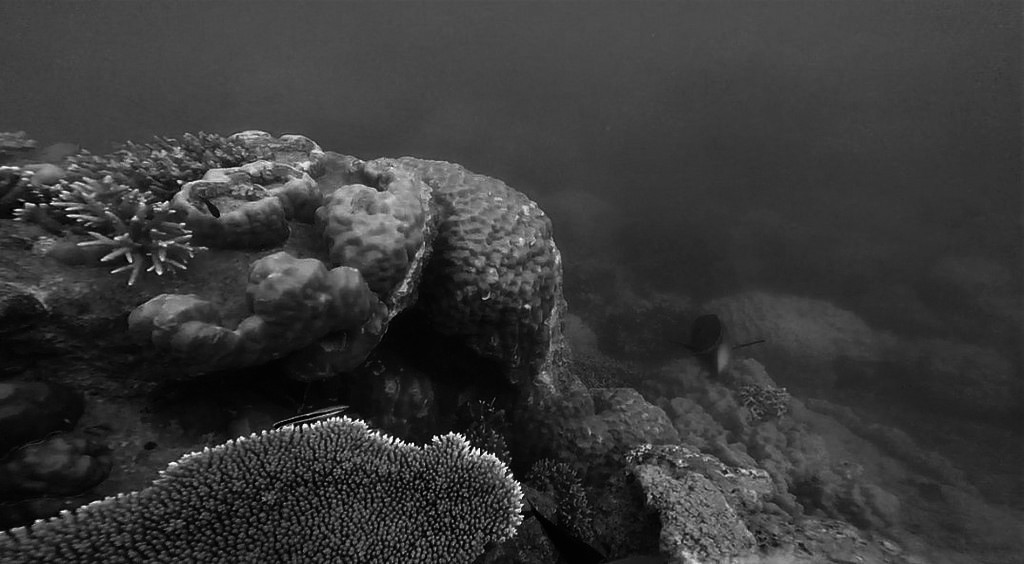
\includegraphics[width=0.2\textwidth]{ocean} &
		\includegraphics[width=0.2\textwidth]{mogrify} \\
	before & after \\
\end{tabular}
\vspace*{3mm}

\subsection{Dropout}
Inspired by the concept of dropout layers in neural networks\footnote{See Srivastava et al.: http://jmlr.org/papers/volume15/srivastava14a.old/srivastava14a.pdf},
which randomly remove nodes in the neural network
to prevent overfitting, we implemented an algorithm
that randomly removes percentage $p$ of the pixels
in an image. It does this by removing
some percentage $p$ of the columns and the same percentage $p$ of the pixels
from each of the remaining columns.

We implemented this algorithm with $p=0.2,0.5$, where $p$ is a value between $0$ and $1$.
In figure 5 the results of putting an image of a tiger through dropout
with $p=0.2$ and $p=0.5$ can be considered.

\vspace*{3mm}
\begin{tabular}{c c c}
	\includegraphics[width=0.2\textwidth]{dropouttwenty} &
		\includegraphics[width=0.2\textwidth]{dropoutfifty} \\
	$p=0.2$ & $p=0.5$ \\
\end{tabular}

\vspace*{3mm}

\section{CLASSIFICATION}

\subsection{Before Compression}

Google Cloud Vision assigned each image a set of labels.
All of the labels assigned to the color images were
accurate or close to accurate, and for each color image,
at least one label closely identified the image (e.g. \textquote{tiger}
for the iamge of a tiger and \textquote{tower} for the image of
the Tokyo Tower).

However, all of the 22 grayscale images were mis-labeled as \textquote{monochrome
photography,} 9 of them were not closely identified, and 4 of them
were only given incorrect labels.

\subsection{After Compression}

\vspace*{2mm}

\begin{tabular}{|c|c|c|}
\hline
{\bf method of} & {\bf fraction of} &
	{\bf fraction of images} \\
{\bf compression} & {\bf images given} & {\bf given the most accurate} \\
{} & {\bf a subset of} & {\bf label given to their} \\
{} & {\bf correct labels} & {\bf un-compressed versions} \\
\hline
mogrify & 18/22 & 15/22 \\
\hline
dropout (20\%) & 17/22 & 15/22 \\
\hline
dropout (50\%) & 13/22 & 8/22 \\
\hline
pooling (16x16) & 20/22 & 14/22 \\
\hline
pooling (32x32) & 9/22 & 4/22 \\
\hline
pooling (64x64) & 1/22 & 0/22 \\
\hline
PCA (25) & 21/22 & 18/22 \\
\hline
PCA (10) & 17/22 & 9/22 \\
\hline
PCA (5) & 6/22 & 0/22 \\
\hline
clustering (8) & 22/22 & 20/22 \\
\hline
clustering (4) & 19/22 & 15/22 \\
\hline
\end{tabular}

\vspace*{2mm}
(Note: this table only analyzes the color images.)
\vspace*{2mm}


\vspace*{2mm}

\begin{tabular}{|c|c|c|}
\hline
{\bf method of} & {\bf fraction of} &
	{\bf fraction of images} \\
{\bf compression} & {\bf images given} & {\bf given the most accurate} \\
{} & {\bf a subset of} & {\bf label given to their} \\
{} & {\bf correct labels} & {\bf un-compressed versions} \\
\hline
mogrify & 18/22 & 15/22 \\
\hline
dropout (20\%) & 17/22 & 15/22 \\
\hline
dropout (50\%) & 13/22 & 8/22 \\
\hline
pooling (16x16) & 20/22 & 14/22 \\
\hline
pooling (32x32) & 9/22 & 4/22 \\
\hline
pooling (64x64) & 1/22 & 0/22 \\
\hline
PCA (25) & 21/22 & 18/22 \\
\hline
PCA (10) & 17/22 & 9/22 \\
\hline
PCA (5) & 6/22 & 0/22 \\
\hline
clustering (8) & 22/22 & 20/22 \\
\hline
clustering (4) & 19/22 & 15/22 \\
\hline
\end{tabular}

\vspace*{2mm}
(Note: this table only analyzes the greyscale images.)
\vspace*{2mm}

As expected, the less the image was compressed, the more accurate
the labels it was assigned were. In addition, larger images
had significantly higher accuracy rates than smaller images.

From the data, it appears that k-means clustering was
the best compression method in terms of maintaining the legibility
of the images for Google Cloud Vision. In a sense, this makes
sense, because posterization generally simplifies images while
retaining the overall shapes in the images.

In future analyses, it may be helpful to estalish a more
specific definition of accuracy and a way to compare
the accuracy of Google Cloud Vision when classifying
images before and after compression, as the table
above does not consider a number of factors, such as
the certainty of different labels, and the number
of completely incorrect labels assigned to images.

\section{CONCLUSIONS}

This information
is useful because data reduction has been used as a method to fight
adversarial attacks, in which stickers, random noise, etc. are added to images,
causing neural networks to misclassify them.\footnote{https://openreview.net/pdf?id=S10qYwywf}
\footnote{https://www.researchgate.net/publication/315890594\_Dimensionality\_ Reduction\_as\_a\_Defense\_against\_Evasion\_Attacks\_on\_Machine\_ Learning\_Classifiers}
For exmaple, putting adversarial stickers on stop signs
can cause neural networks to be unable to detect stop signs.\footnote{http://bair.berkeley.edu/blog/2017/12/30/yolo-attack/}
The amount by which one can compress an image before it becomes
illegible to neural networks, as well as the best method to use to compress an
image to maintain legibility, can inform methods that use data reduction
to fight adversarial attacks.

\addtolength{\textheight}{-12cm}   % This command serves to balance the column lengths
                                  % on the last page of the document manually. It shortens
                                  % the textheight of the last page by a suitable amount.
                                  % This command does not take effect until the next page
                                  % so it should come on the page before the last. Make
                                  % sure that you do not shorten the textheight too much.

%%%%%%%%%%%%%%%%%%%%%%%%%%%%%%%%%%%%%%%%%%%%%%%%%%%%%%%%%%%%%%%%%%%%%%%%%%%%%%%%

\section*{ACKNOWLEDGMENT}

We would like to thank Prof. Strang for his support and interesting and informative lectures.

%%%%%%%%%%%%%%%%%%%%%%%%%%%%%%%%%%%%%%%%%%%%%%%%%%%%%%%%%%%%%%%%%%%%%%%%%%%%%%%%
\begin{thebibliography}{99}

\bibitem{c1} \textquote{Cloud Vision API.} Google Cloud. https://cloud.google.com/vision/
\bibitem{c2} \textquote{Pooling.} UFLDL Tutorial. http://ufldl.stanford.edu/tutorial/supervised/Pooling/
\bibitem{c3} \textquote{mogrify.} ImageMagick. https://www.imagemagick.org/script/mogrify.php
\bibitem{c4} \textquote{command line options.} ImageMagick. https://www.imagemagick.org/script/command-line-options.php\#quality
\bibitem{c5} Gopalakrishnan, Soorya, et. al. \textquote{Combating Adversarial
	Attacks Using Sparse Representations.} ICLR 2018. https://openreview.net/pdf?id=S10qYwywf
\bibitem{c6} Bhagoji, Arjun, et. al. \textquote{Dimensionality Reduction as a Defense against Evasion Attacks on Machine Learning Classifiers.} https://www.researchgate.net/publication/315890594\_Dimensionality\_ Reduction\_as\_a\_Defense\_against\_Evasion\_Attacks\_on\_Machine\_ Learning\_Classifiers
\bibitem{c7} Evtimov, Ivan, et. al. \textquote{Physical Adversarial Examples Against Deep
	Learning Networks.} Berkeley Artificial Intelligence Research. Published 30 December 2017. http://bair.berkeley.edu/blog/2017/12/30/yolo-attack/

\end{thebibliography}

\end{document}
